% This file should be saved as crimping.tex in the P1 folder
% as referenced in the main document's \section{Pendahuluan}
\subsection{Latar Belakang}
IPSec dibuat untuk kebutuhan melindungi data sensitif yang dikirim melalui jaringan-jaringan publik seperti internet. Teknologi seperti VPN menggunakan IPSec pada dasarnya, dan memungkinkan pengiriman data antar lokasi, misalnya kantor pusat ke cabang secara aman dan efisien.

\subsection{Dasar Teori}
IPSec atau Internet Protocol Security adalah protokol keamanan yang digunakan untuk mengamankan komunikasi data melalui jaringan IP dengan mengenkripsi dan mengotentikasi paket -paket data, layaknya sebuah VPN. IPSec terdiri dari dua fase, yaitu IKE Phase 1 dan Phase 2. IKE Phase 1 membentuk saluran terenkrpsi kedua end point, dan IKE Phase 2 menghandle parameter untuk mengamankan data, seperti algoritma enkripsi dan/atau metode autentikasi.

%===========================================================%
\section{Tugas Pendahuluan}
Bagian ini berisi jawaban dari tugas pendahuluan yang telah anda kerjakan, beserta penjelasan dari jawaban tersebut
\begin{enumerate}
	\item Pada IKE Phase 1, fase ini mempersiapkan saluran yang aman dan mengautentikasi kedua endpoint. Sedangkan IKE Phase 2 membentuk tunnel IPSec agar transfer data menjadi aman. Parameter keamanan yang harus disepakati meliputi algoritma enkripsi (contohnya AES128), algoritma autentikasi (contohnya HMAC-SHA1), metode autentikasi (contohnya PSK/pre shared keys), diffie-hellman group, lifetime (84600 detik untuk phase 1 dan 3600 detik untuk phase 2)
        \item Parent 100Mbps (GLOBAL), child Elearning 40Mbps prioritas 1,, Child guru dan staf 30Mbps prioritas 2, Siswa 20Mbps prioritas 3, CCTV dan update sistem 10Mbps prioritas 4
        \item Referensi: Cisco Community – IPsec Tunnel: Understanding Phase 1 and 2; NetworkLessons – IPsec (Internet Protocol Security); MikroTik Docs – IPsec and Site-to-Site Example; MikroTik Docs – Queues and PCQ Example .
\end{enumerate}

\section{Langkah-Langkah Percobaan}
Dalam percobaan crimping dan routing IPv4, kami memulai dengan mempersiapkan peralatan yang dibutuhkan, seperti kabel UTP, konektor RJ45, tang crimping, dan LAN tester. Kami menyusun kabel UTP dengan mengikuti urutan warna yang benar sesuai standar T568B untuk memastikan koneksi yang tepat. 

\begin{figure}[H]
    \centering
    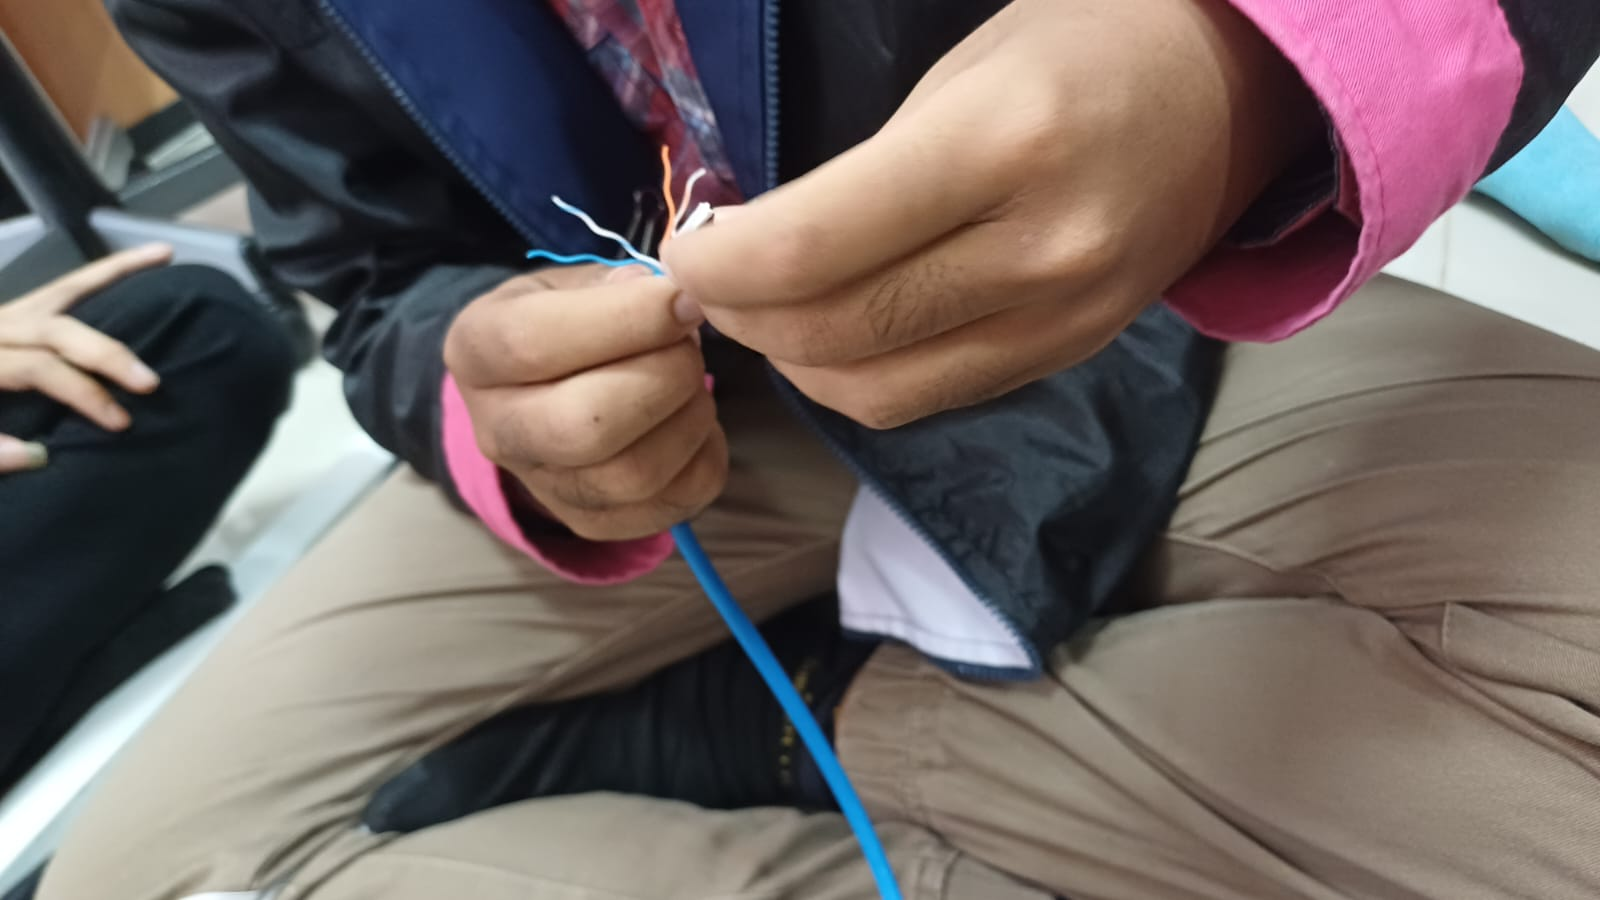
\includegraphics[width=0.48\textwidth]{P1/img/Crimping 1.jpeg}
    \caption{Proses penyusunan kabel}
    \label{fig:crimping1}
\end{figure}

Setelah itu, kami menggunakan tang crimping untuk memasang konektor RJ45 pada ujung kabel. 

\begin{figure}[H]
    \centering
    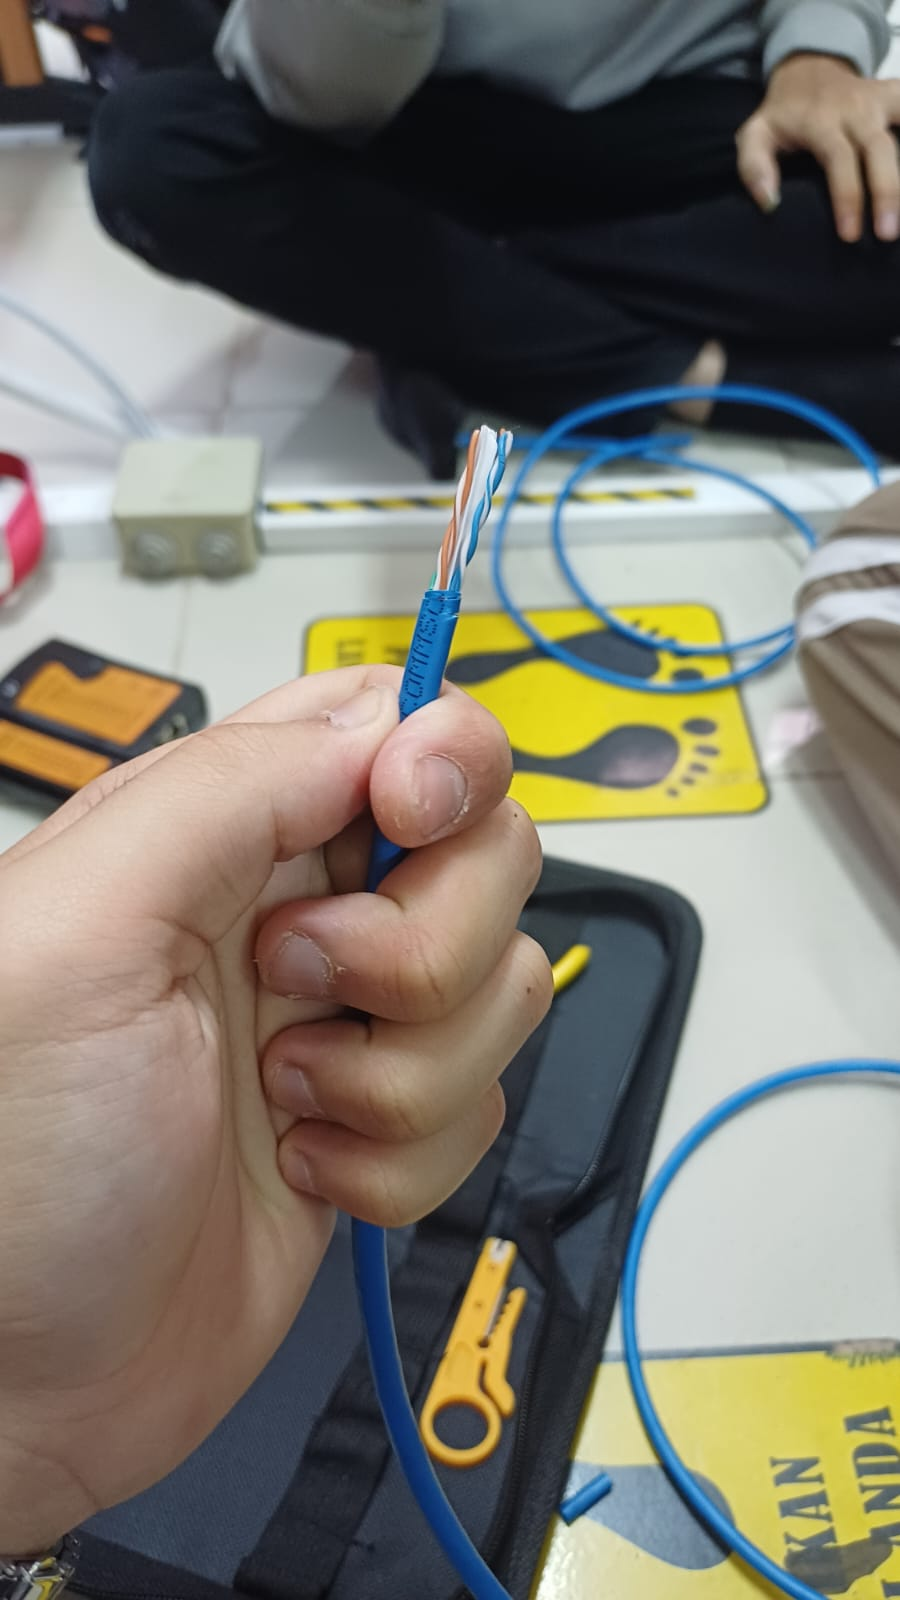
\includegraphics[width=0.48\textwidth]{P1/img/Crimping 2.jpeg}
    \caption{Kabel sudah tersusun sebelum crimping}
    \label{fig:crimping2}
\end{figure}

Untuk memverifikasi hasil crimping, kami menguji kabel dengan LAN tester untuk memastikan bahwa setiap kabel terhubung dengan benar. 

\begin{figure}[H]
    \centering
    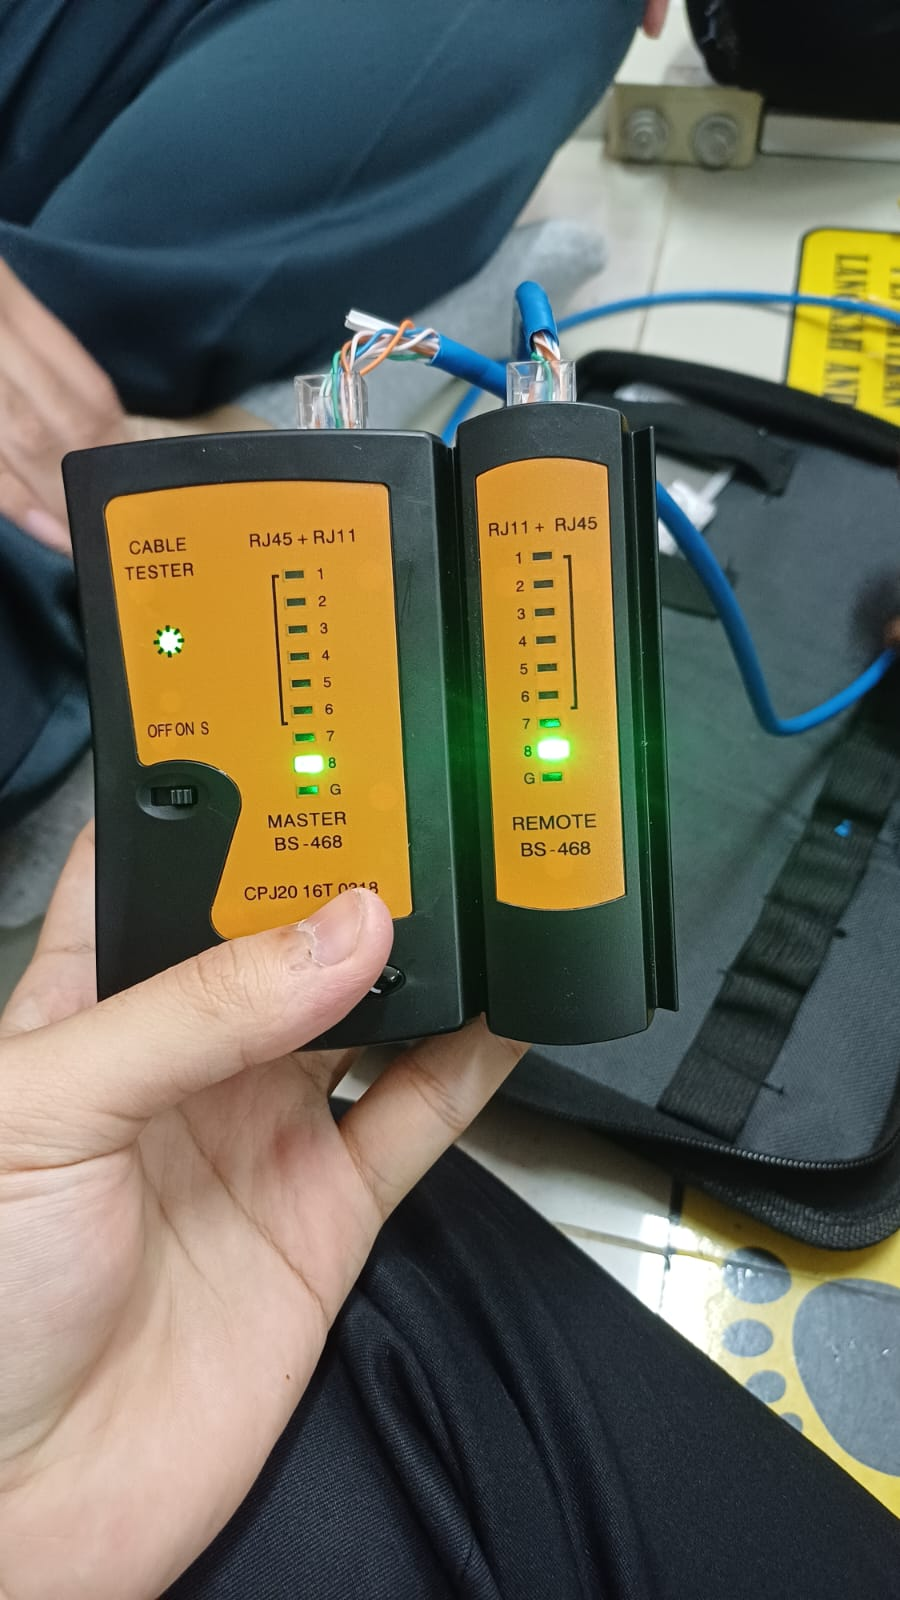
\includegraphics[width=0.48\textwidth]{P1/img/Crimping 3.jpeg}
    \caption{Percobaan kabel dengan LAN Tester}
    \label{fig:crimping3}
\end{figure}

Kabel hasil crimping yang telah selesai 

\begin{figure}[H]
    \centering
    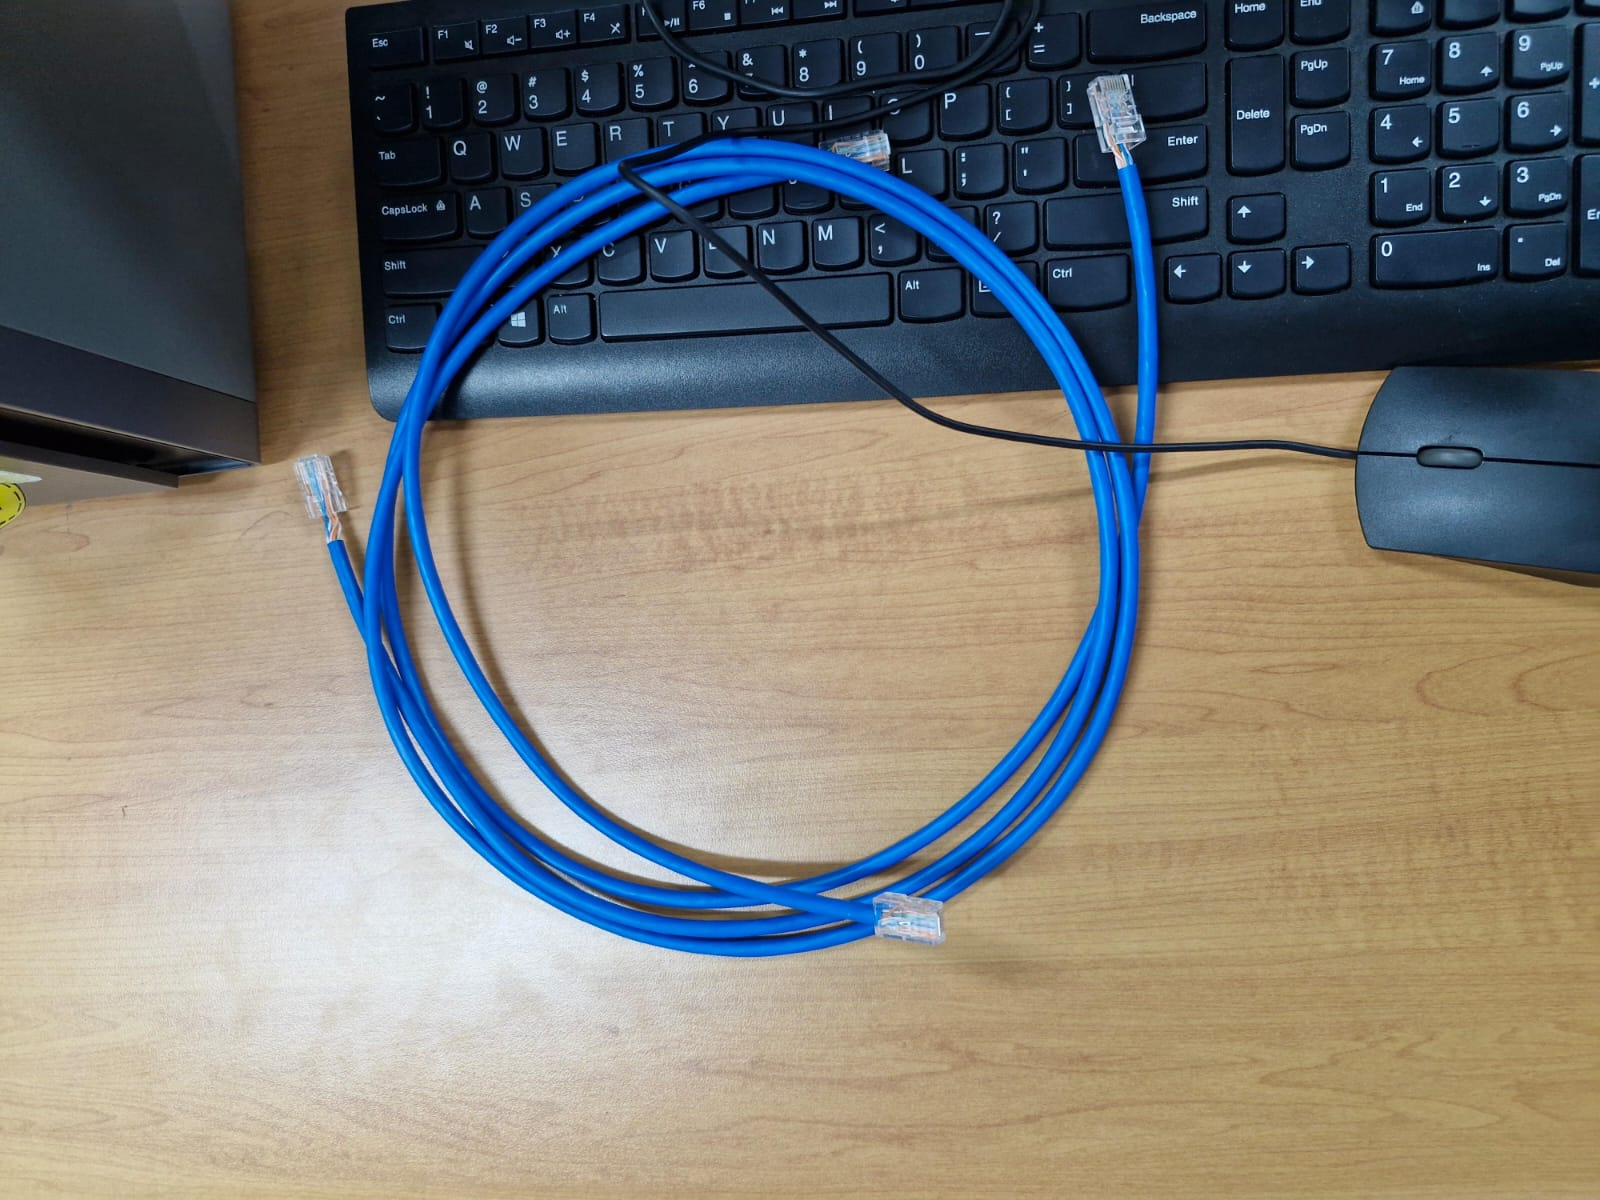
\includegraphics[width=0.48\textwidth]{P1/img/Crimping 4.jpeg}
    \caption{Foto Kabel}
    \label{fig:crimping4}
\end{figure}

\newpage
Pada percobaan Routing IPv4 menggunakan aplikasi Winbox, saya memulai dengan mereset kedua router ke kondisi awal untuk menghindari konflik konfigurasi. Langkah pertama adalah membuka aplikasi Winbox dan login ke kedua router menggunakan MAC address atau IP default, dengan username "admin" dan tanpa password jika belum diatur. Setelah login berhasil, saya mengonfigurasi IP address pada interface ether1 yang digunakan untuk menghubungkan kedua router. Pada router pertama, saya memberikan IP address 10.10.10.1/30, dan pada router kedua saya memberikan IP address 10.10.10.2/30. Setelah itu, saya melanjutkan dengan mengonfigurasi interface ether2 yang akan digunakan untuk menghubungkan router dengan jaringan LAN. Pada router pertama, saya memberikan IP address 192.168.10.1/27, sementara pada router kedua saya memberikan IP address 192.168.20.1/27 untuk jaringan LAN masing-masing. 

Selanjutnya, saya menambahkan routing statis untuk memastikan paket data dapat diteruskan antar router. Saya membuka menu IP -> Routes di Winbox, kemudian menambahkan rute untuk masing-masing router. Pada router pertama, saya menambahkan rute dengan Dst. Address 192.168.20.0/27 dan gateway 10.10.10.2, sementara pada router kedua saya menambahkan rute dengan Dst. Address 192.168.10.0/27 dan gateway 10.10.10.1. Setelah konfigurasi routing selesai, saya mengonfigurasi IP address secara manual pada laptop yang terhubung ke kedua router. Laptop yang terhubung ke router pertama saya berikan IP address 192.168.10.2 dengan gateway 192.168.10.1, sedangkan laptop yang terhubung ke router kedua saya berikan IP address 192.168.20.2 dengan gateway 192.168.20.1. 

Terakhir, saya melakukan ping untuk menguji konektivitas dari laptop yang terhubung ke router pertama ke laptop yang terhubung ke router kedua. Jika ping berhasil, itu berarti konfigurasi routing IPv4 telah berhasil dan komunikasi antar router berjalan dengan baik.

\newpage
\subsection*{Percobaan Statis (Gagal)}
\begin{figure}[H]
  \centering
  \begin{minipage}[t]{0.48\textwidth}
    \centering
    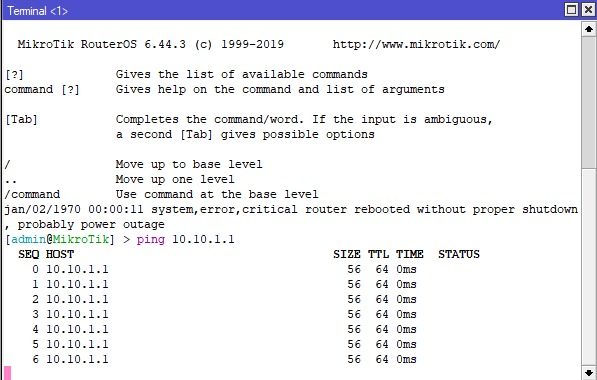
\includegraphics[width=\linewidth]{P1/img/PC1->Router1.jpeg}
    \caption{PC 1 -> Router 1}
    \label{fig:pc1router1}
  \end{minipage}
  \hfill
  \begin{minipage}[t]{0.48\textwidth}
    \centering
    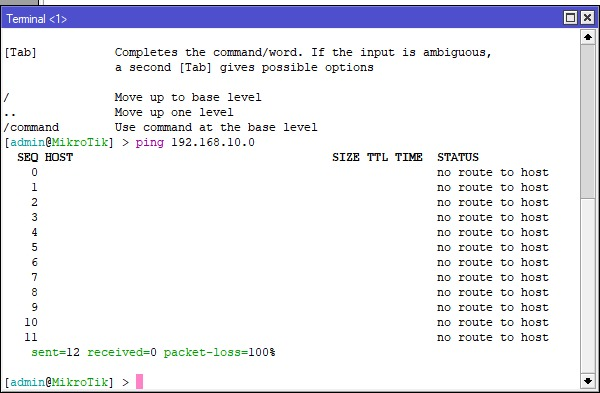
\includegraphics[width=\linewidth]{P1/img/Router1->Router2.jpeg}
    \caption{Router 1 -> Router 2}
    \label{fig:router1router2}
  \end{minipage}
\end{figure}

\begin{figure}[H]
  \centering
  \begin{minipage}[t]{0.48\textwidth}
    \centering
    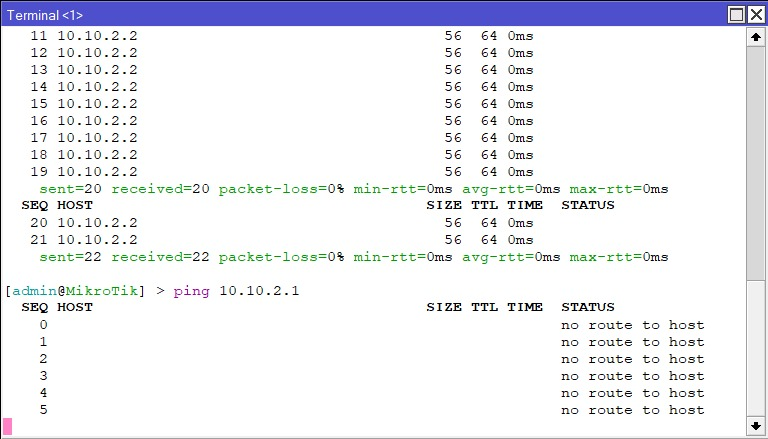
\includegraphics[width=\linewidth]{P1/img/Router2->Router1.jpeg}
    \caption{Router 2 -> Router 1}
    \label{fig:router2router1}
  \end{minipage}
  \hfill
  \begin{minipage}[t]{0.48\textwidth}
    \centering
    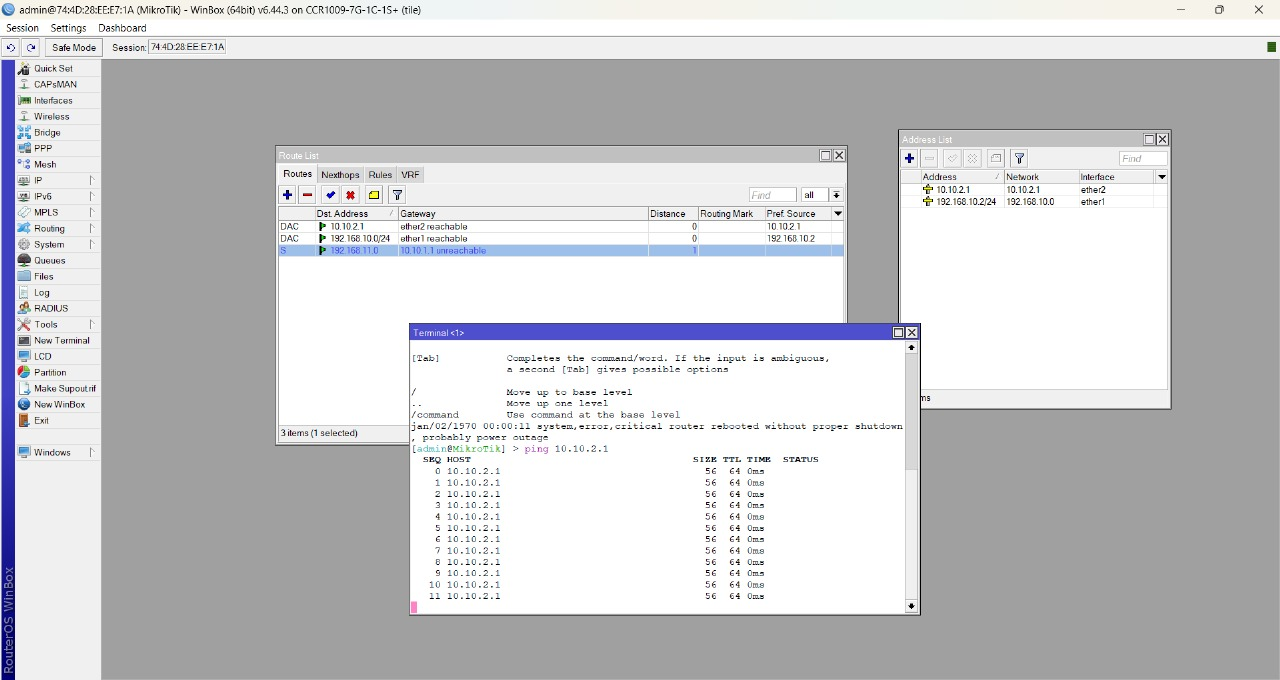
\includegraphics[width=\linewidth]{P1/img/PC2->Router2.jpeg}
    \caption{PC 2 -> Router 2}
    \label{fig:pc2router2}
  \end{minipage}
  \caption*{Proses percobaan Routing IPv4}
\end{figure}

\newpage
\section{Analisis Hasil Percobaan}

Pada percobaan Crimping, kami berhasil melaksanakan proses crimping kabel dengan menggunakan alat yang telah disiapkan, namun pada kabel LAN pertama, kami menemui kendala karena urutan kabel yang tidak sesuai standar, yang menyebabkan koneksi tidak terhubung dengan baik. Hal ini mengharuskan kami untuk mengulang proses crimping, dengan memotong kabel tersebut dan menyusunnya kembali sesuai urutan warna yang benar. Setelah melakukan pengulangan pada percobaan kedua, kabel berhasil terpasang dengan benar dan koneksi pun berjalan lancar.

Untuk percobaan Routing IPv4, kami mengalami kendala dalam melaksanakan konfigurasi IPv4 statis. Meskipun kami telah mengikuti prosedur yang benar, kami tidak berhasil menyelesaikan percobaan ini hingga waktu habis. Masalah utama yang kami temui adalah kesalahan pada pengaturan alamat IP, di mana pada laptop kedua yang terhubung dengan router kedua, terdapat alamat IP bawaan dari Google yang tidak dapat dihapuskan, yang menyebabkan koneksi terus terinterupsi. Hal ini menghambat komunikasi antar perangkat, sehingga konfigurasi statis tidak dapat berhasil. Selain itu, kami juga mencoba untuk melaksanakan routing IPv4 dinamis, namun karena waktu yang terbatas, kami tidak dapat menyelesaikan percobaan ini. Dengan waktu yang hampir habis, kami tidak dapat mengonfigurasi routing dinamis menggunakan protokol RIP yang direncanakan.

\newpage
\section{Hasil Tugas Modul}
Dalam praktikum ini, saya membangun jaringan internal untuk sebuah perusahaan dengan membagi jaringan berdasarkan departemen-departemen yang ada. Setiap departemen memiliki jaringan lokalnya sendiri yang terhubung melalui satu router utama. Untuk mempermudah pengelolaan, saya memutuskan untuk menghubungkan satu komputer yang mewakili sepuluh perangkat end user, karena menghubungkan lebih dari seratus perangkat akan menghabiskan waktu dan sumber daya.

Proses dimulai dengan menyiapkan sebuah router yang menghubungkan dua switch utama. Switch di sisi kiri router saya hubungkan dengan departemen Produksi dan Administrasi, sedangkan switch di sisi kanan menghubungkan departemen Keuangan dan R\&D. Router saya konfigurasi dengan menggunakan alamat IP 192.168.1.1 untuk interface g0/0 yang terhubung ke switch kiri, dan alamat IP 192.168.2.1 untuk interface g0/1 yang terhubung ke switch kanan. Setelah itu, saya melakukan alokasi IP untuk masing-masing departemen:
untuk Produksi menggunakan IP 192.168.1.51 hingga 192.168.1.100, Administrasi menggunakan 192.168.1.21 hingga 192.168.1.40, Keuangan menggunakan 192.168.2.11 hingga 192.168.2.20, dan R\&D menggunakan 192.168.2.101 hingga 192.168.2.200.

Selanjutnya, saya melakukan percobaan pengiriman pesan antar end user untuk menguji konektivitas antar departemen. Saya mencoba mengirim pesan dari PC di departemen Produksi ke departemen Keuangan dan R\&D, serta sebaliknya dari PC Keuangan dan R\&D ke departemen Administrasi. Hasilnya, pesan berhasil dikirim dan diterima dengan sukses, yang menunjukkan bahwa konfigurasi jaringan dan routing yang saya buat berfungsi dengan baik.

\begin{figure}[H]
  \centering
  \begin{minipage}[t]{0.48\textwidth}
    \centering
    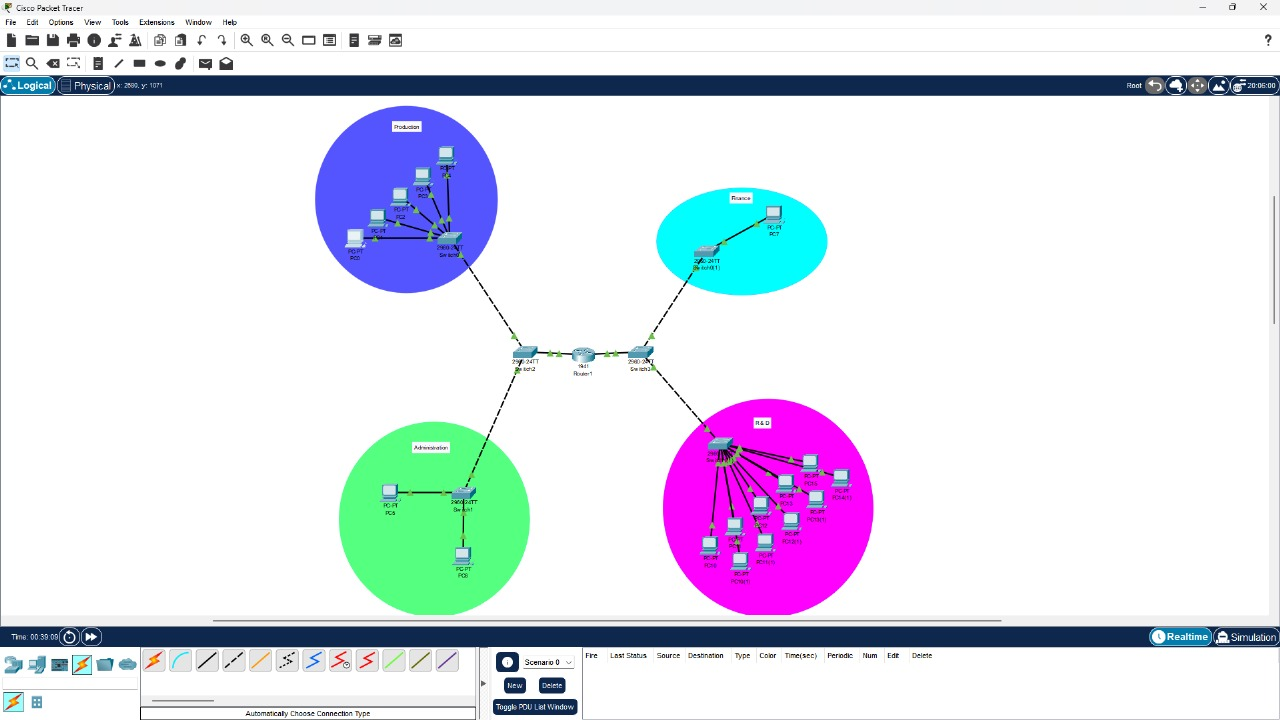
\includegraphics[width=\linewidth]{P1/img/Struktur.jpeg}
    \caption{Struktur Jaringan Keseluruhan}
    \label{fig:struktur}
  \end{minipage}
  \hfill
  \begin{minipage}[t]{0.48\textwidth}
    \centering
    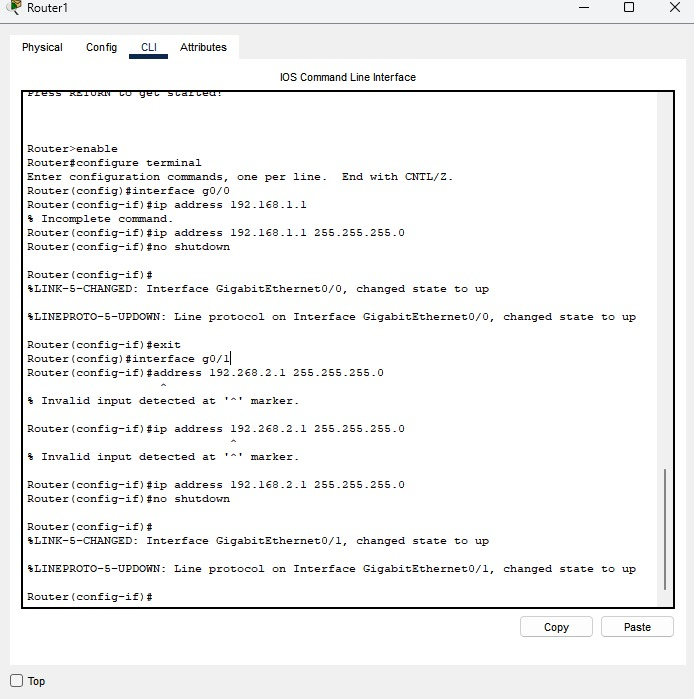
\includegraphics[width=\linewidth]{P1/img/CLI Config.jpeg}
    \caption{CLI Router Utama}
    \label{fig:cli}
  \end{minipage}
\end{figure}

\newpage
\section{Struktur Jaringan}

\begin{figure}[H]
  \centering
  \begin{minipage}[t]{0.48\textwidth}
    \centering
    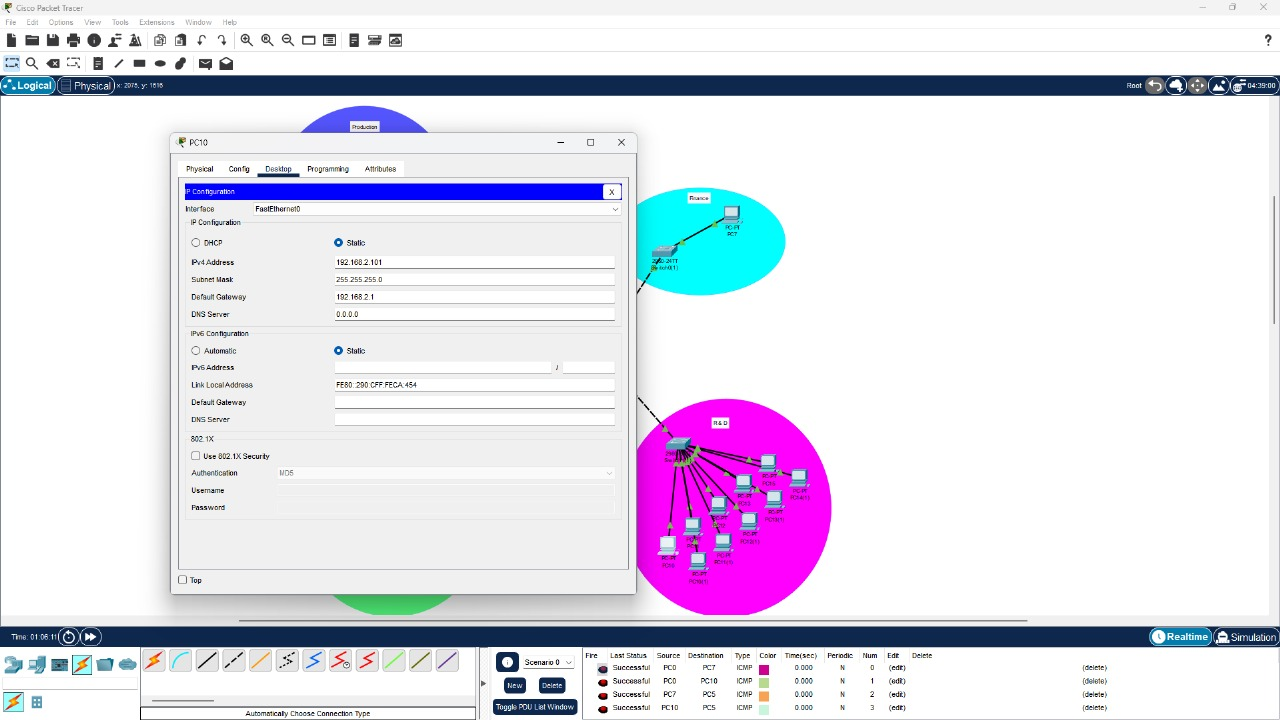
\includegraphics[width=\linewidth]{P1/img/R&DIP.jpeg}
    \caption{Address R\&D}
    \label{fig:rnd}
  \end{minipage}
  \hfill
  \begin{minipage}[t]{0.48\textwidth}
    \centering
    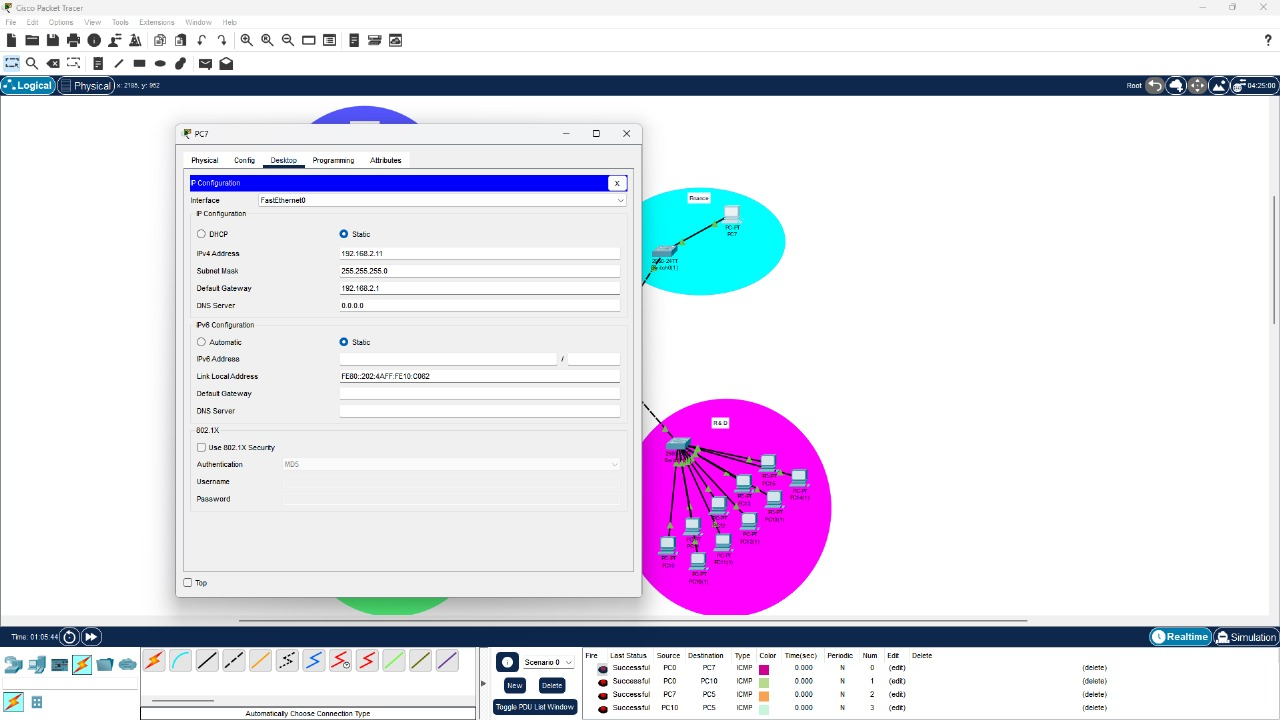
\includegraphics[width=\linewidth]{P1/img/FinIP.jpeg}
    \caption{Address Finance}
    \label{fig:finance}
  \end{minipage}
\end{figure}

\newpage
\section{Jaringan Bagian Kanan}

\begin{figure}[H]
  \centering
  \begin{minipage}[t]{0.48\textwidth}
    \centering
    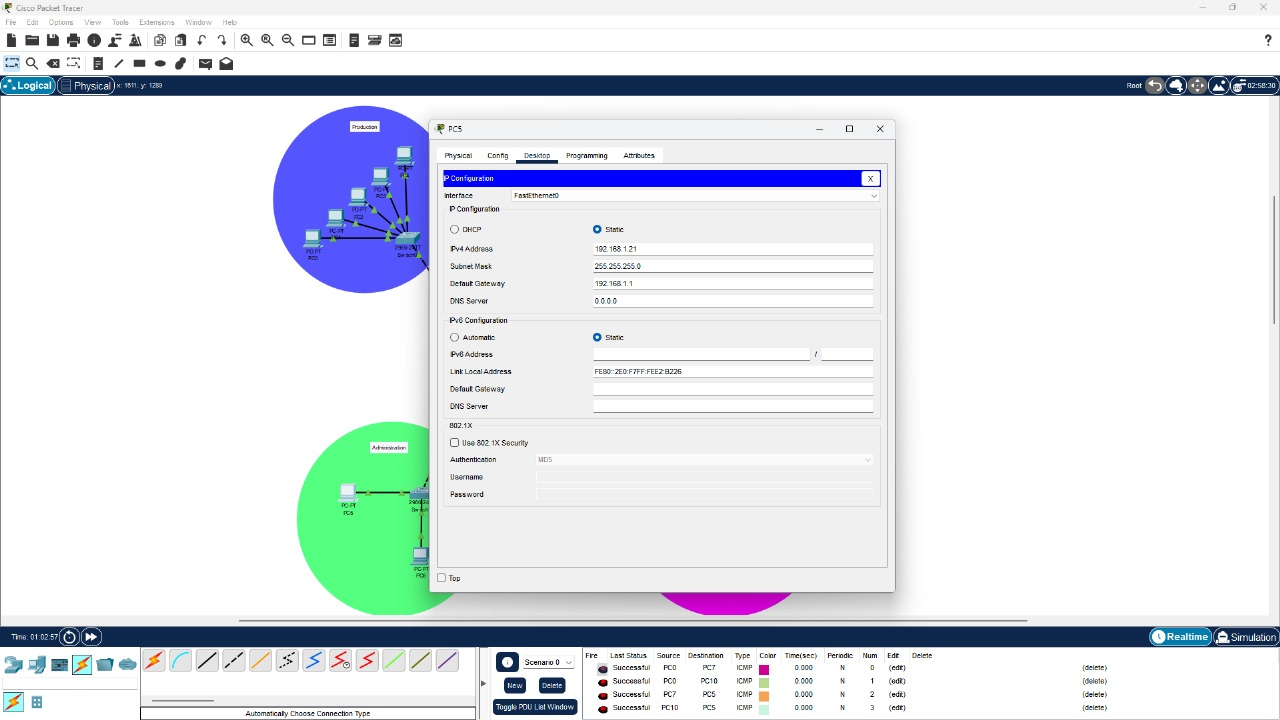
\includegraphics[width=\linewidth]{P1/img/ProdIP.jpeg}
    \caption{Address Production}
    \label{fig:production}
  \end{minipage}
  \hfill
  \begin{minipage}[t]{0.48\textwidth}
    \centering
    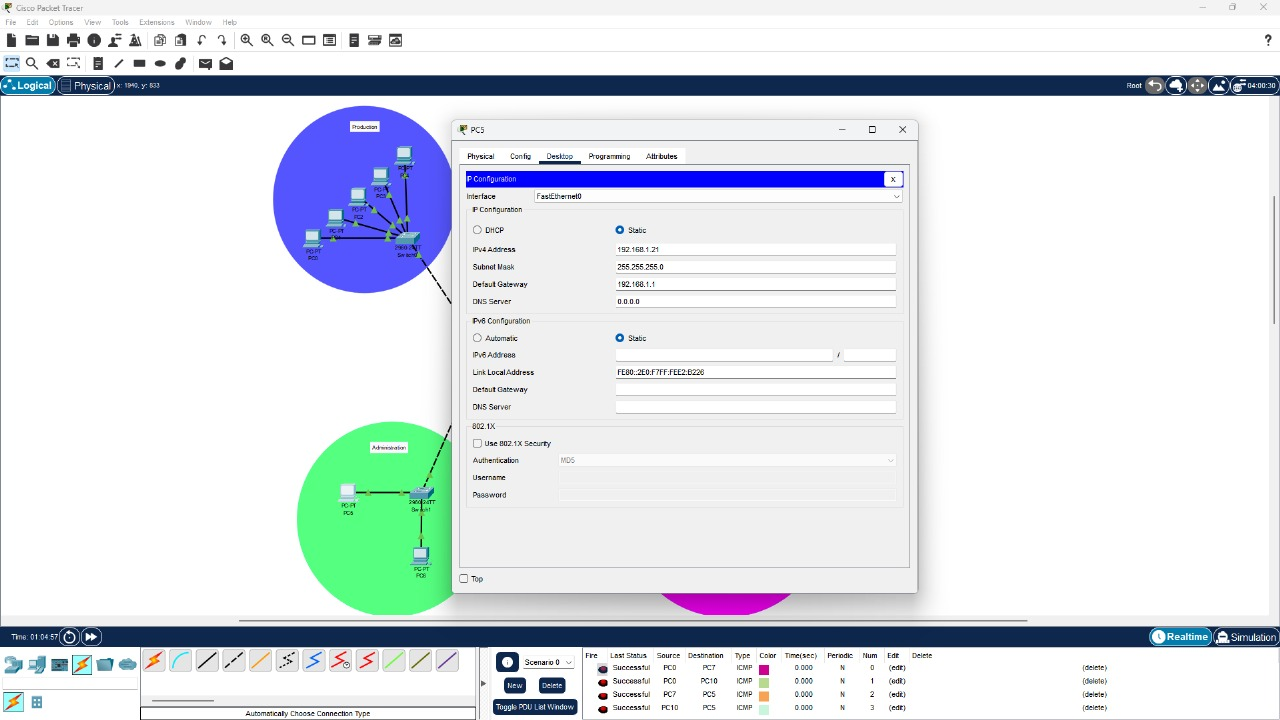
\includegraphics[width=\linewidth]{P1/img/AdminIP.jpeg}
    \caption{Address Administration}
    \label{fig:admin}
  \end{minipage}
\end{figure}

\begin{figure}[H]
  \centering
  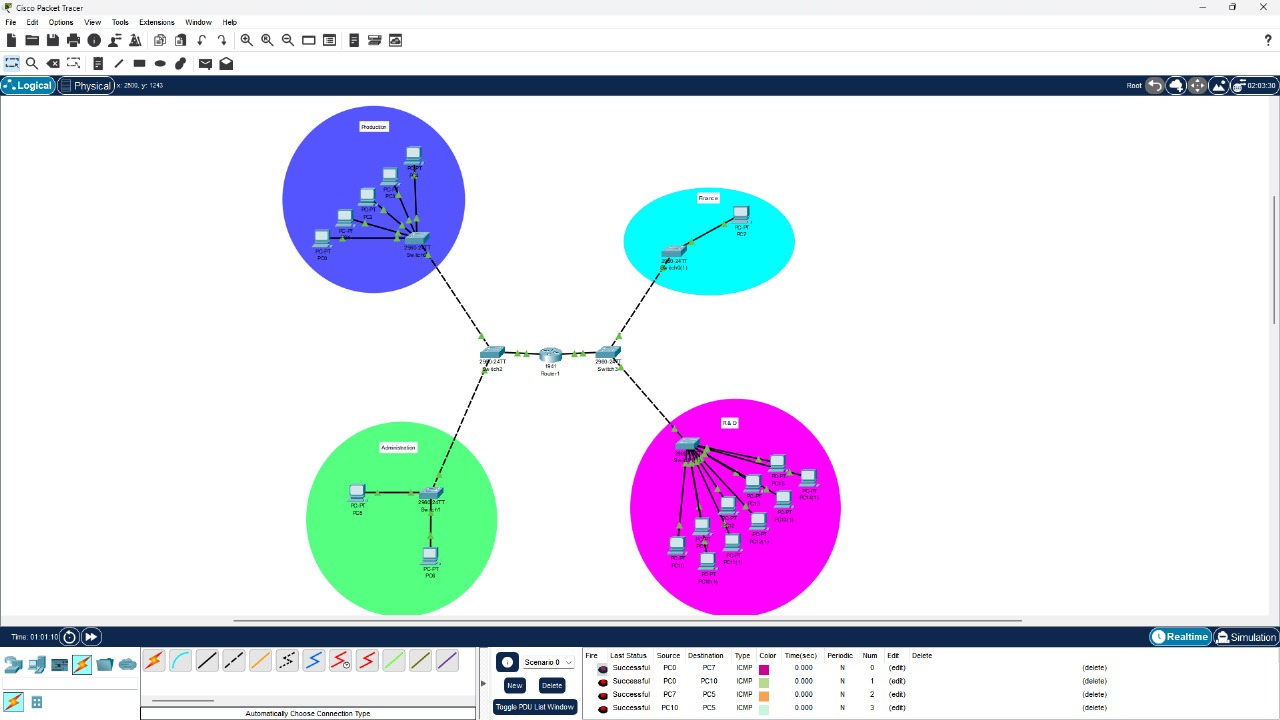
\includegraphics[width=0.48\textwidth]{P1/img/Connected.jpeg}
  \caption{Seluruh Jaringan terkoneksi}
  \label{fig:connected}
\end{figure}

\newpage
\section{Lampiran}
\subsection{Dokumentasi saat praktikum}

\begin{figure}[H]
    \centering
    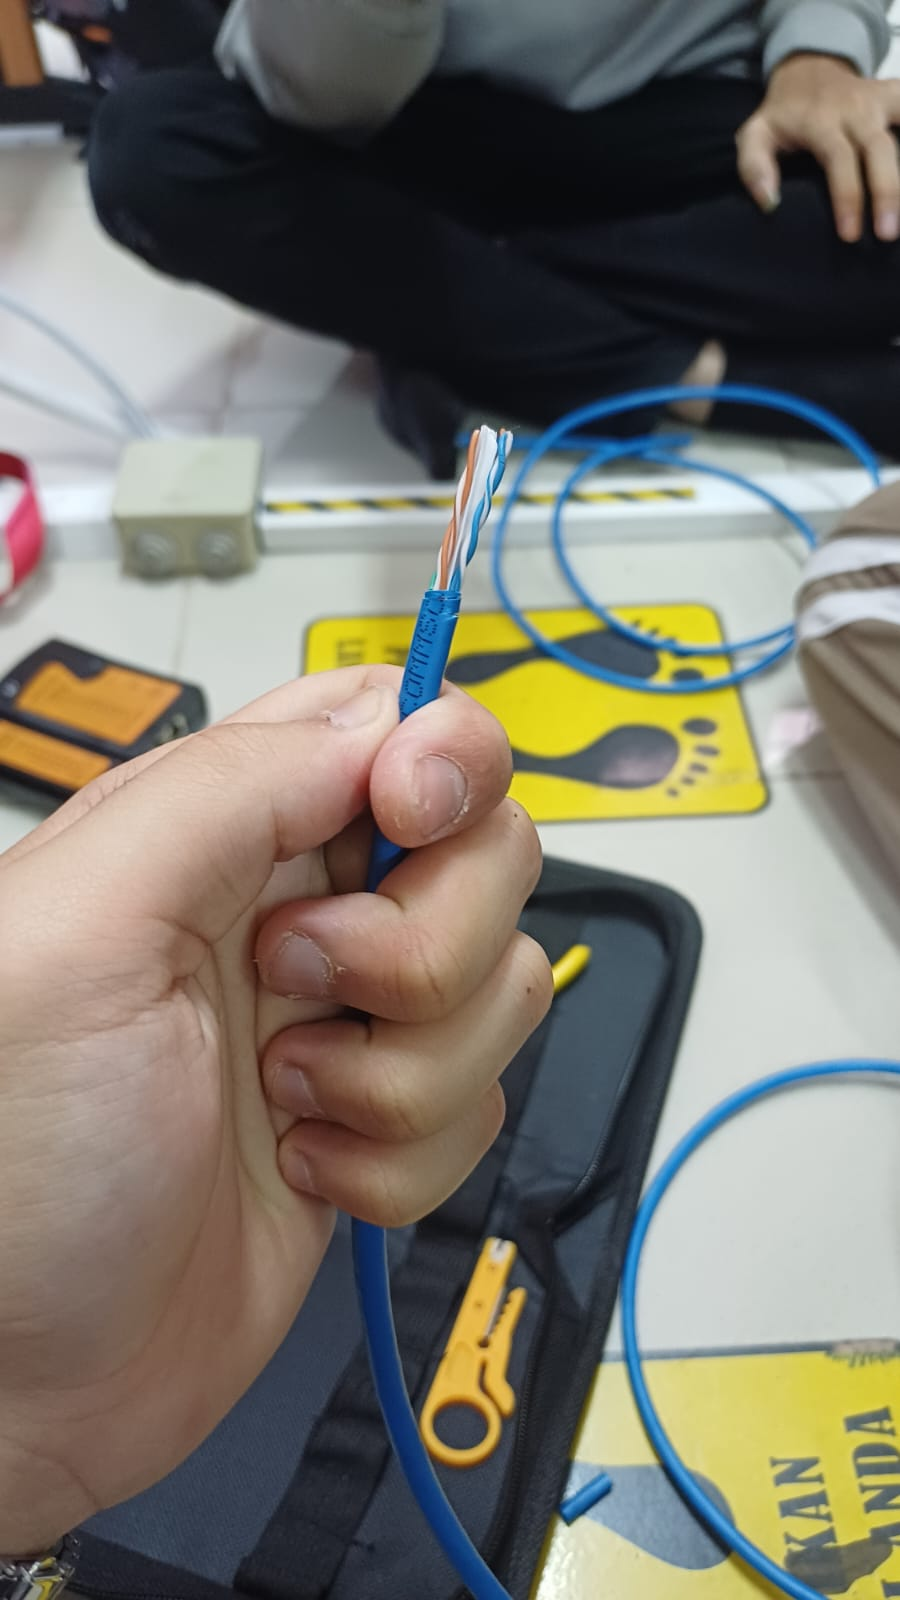
\includegraphics[width=0.48\textwidth]{P1/img/Crimping 2.jpeg}
    \caption{Kabel sudah tersusun sebelum crimping}
    \label{fig:crimping2_lampiran}
\end{figure}

Untuk memverifikasi hasil crimping, kami menguji kabel dengan LAN tester untuk memastikan bahwa setiap kabel terhubung dengan benar. 

\begin{figure}[H]
    \centering
    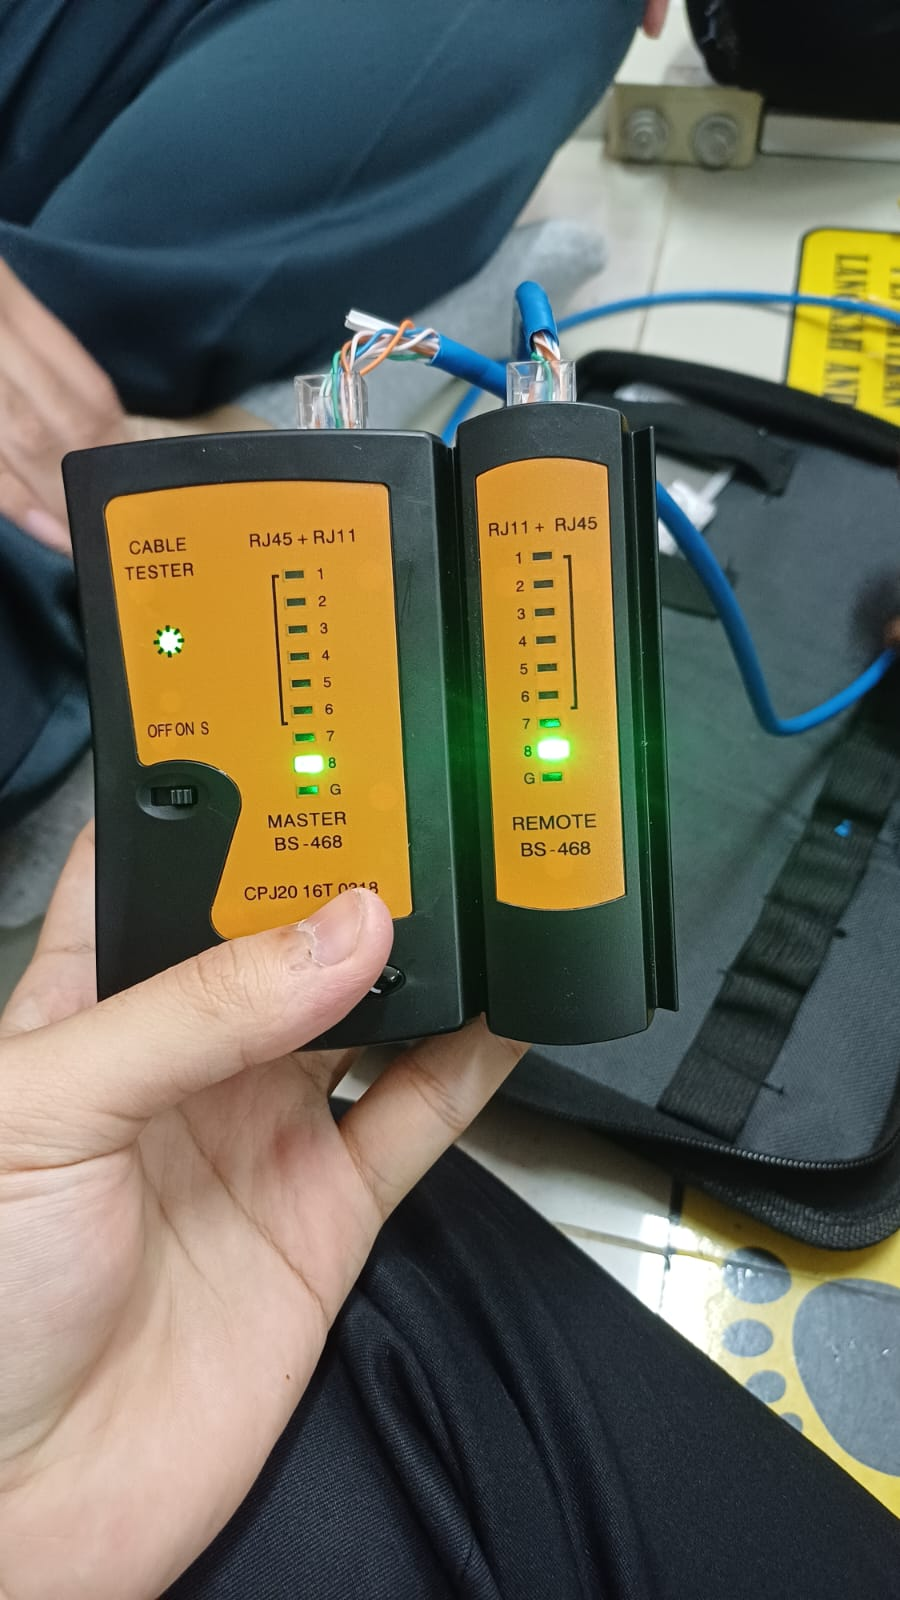
\includegraphics[width=0.48\textwidth]{P1/img/Crimping 3.jpeg}
    \caption{Percobaan kabel dengan LAN Tester}
    \label{fig:crimping3_lampiran}
\end{figure}

Kabel hasil crimping yang telah selesai 

\begin{figure}[H]
    \centering
    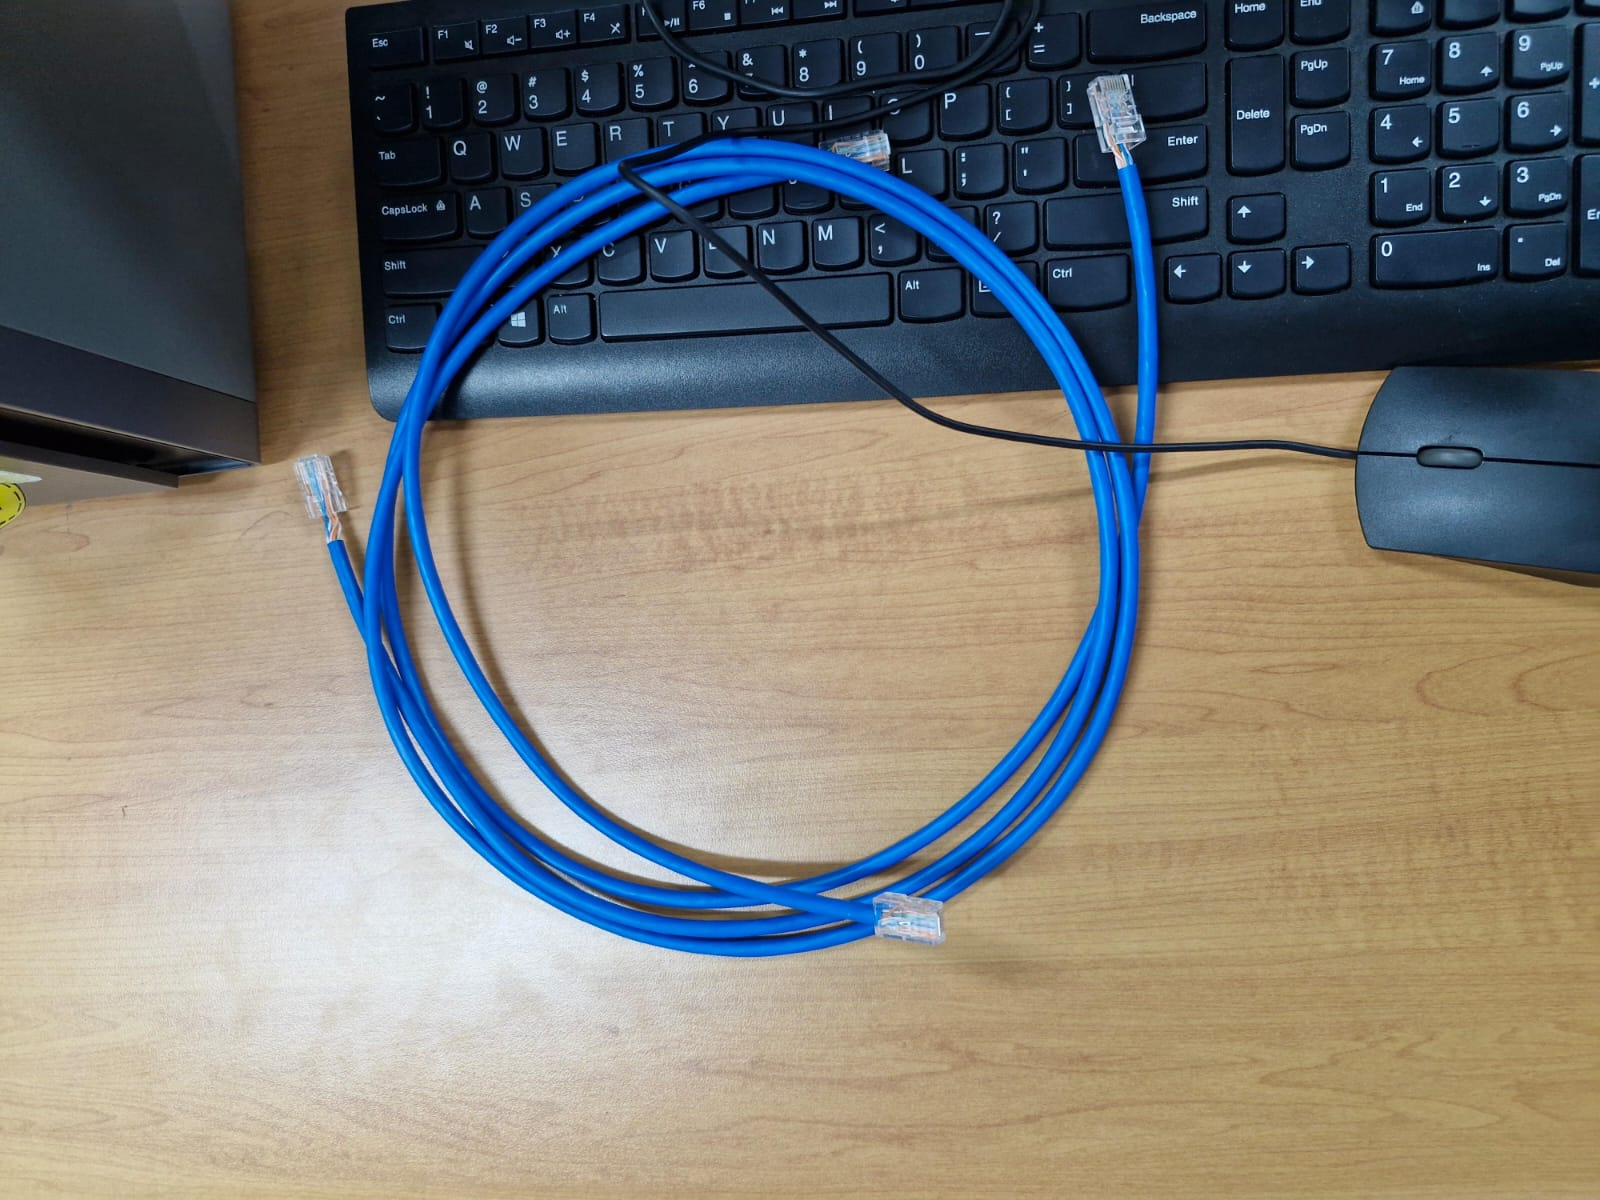
\includegraphics[width=0.48\textwidth]{P1/img/Crimping 4.jpeg}
    \caption{Foto Kabel}
    \label{fig:crimping4_lampiran}
\end{figure}


